%\documentclass{jsarticle}

%\usepackage{amsmath, amssymb}%数式
%\usepackage{array, booktabs}%表成型
%\usepackage[dvipdfmx]{graphicx}%画像

%\begin{document}

\subsection{解析手法B}
\label{subsec:PSAnalyses}

\subsubsection{使用データ}
\label{subsubsec:PSData}

実験で得られたデータのうち,解析に用いたのは3 日目に磁場標的を用いたランと4 日目に銅板標的を用いたランとの2 つであり,それぞれのデータを表~\ref{tab:PSdata} に示す.
\begin{table}[h]
	\centering
	\caption{PS の解析に用いたデータ}
	\begin{tabular}{ccc} \toprule
	標的の種類 & 磁場$B~[\mathrm{G}]$ & Event 数 \\ \midrule
	銅板標的 & --- & 43502 \\
	磁場標的 & 53.97 & 448073 \\ \bottomrule
	\end{tabular}\label{tab:PSdata}
\end{table}%

なお,磁場標的を用いたデータについては先に述べたように磁場がランの途中で変化していたので,解析には変化後のデータとして,最初の30000~events を除いたデータのみを用いた.
詳しくは\ref{subsubsec:PSMagChangeCheck}で述べる.

\subsubsection{WFD波形の解析}
\label{subsubsec:PSEventDisplay}

WFD (CAEN Waveform Digitizer V1721) で得られたイベント / 波形の例を図~\ref{fig:PSEventDisplayAll}, \ref{fig:PSEventDisplayZoom} に示す.
\begin{figure}[h]
	\centering
	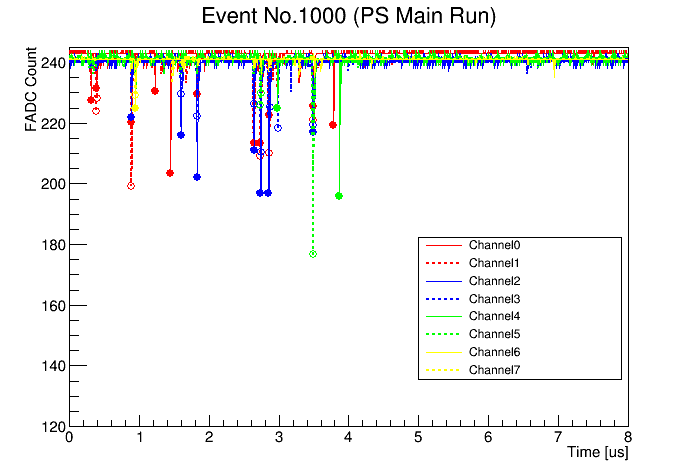
\includegraphics[width = 0.9\textwidth]{figure/odagawa/PSEventDisplayAll.eps}
	\caption{プラスチックシンチレータで得られた波形 ($8~\mu\mathrm{s}$ 全体).線の種類がそれぞれのチャンネルに対応している.}
	\label{fig:PSEventDisplayAll}
\end{figure}%
\begin{figure}[h]
	\centering
	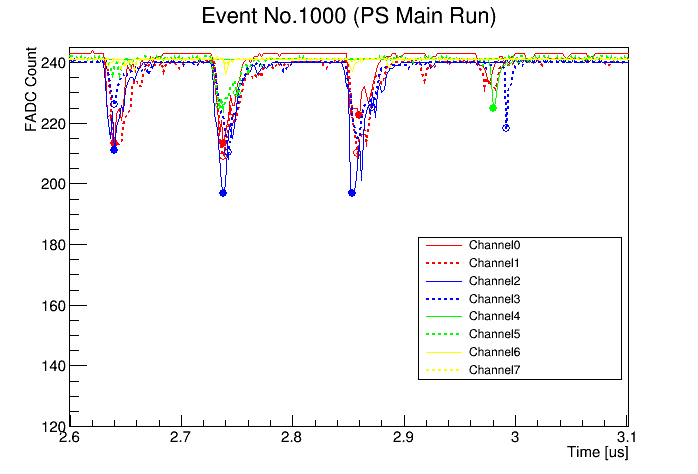
\includegraphics[width = 0.9\textwidth]{figure/odagawa/PSEventDisplayZoom.eps}
	\caption{プラスチックシンチレータで得られた波形 (一部拡大).図~\ref{fig:PSEventDisplayAll} の2.6 - 3.1~$\mu$s を拡大したものである.}
	\label{fig:PSEventDisplayZoom}
\end{figure}%
図~\ref{fig:PSEventDisplayZoom} からもわかる通り,プラスチックシンチレータのデータについては一つの信号が立ち下がる前に次の信号を検出してしまう「パイルアップ」はほとんどないものと考えられる.
また,立ち上がりが十分に早くない場合には,threshold を信号ごとにすべて同じにしたとき,threshold を超える時間が信号の高さで変化し,時刻がきちんと得られないことがある.
このような時刻のずれを補正するためにTQ 補正などが行われることがあるが,図~\ref{fig:PSEventDisplayAll} から信号の立ち上がりは十分早く,そのような補正は必要ないと判断した.
以降ではこれらを考慮したうえで,固定threshold を,プラスチックシンチレータのアフターパルスやベースラインの揺らぎを無視できる大きさ (8~WFD Count, 30~mV相当) に設定して解析を行った.

\subsubsection{ミューオン寿命解析}
\label{subsubsec:PSLife}

まず,銅板標的を用いたランのデータからミューオンの寿命を求めた.
\ref{subsubsec:PSEventDisplay} で述べたようにthreshold を設定し,固定threshold を越えたところから初めてthreshold 以下になるところまでを一つの崩壊$e^{+}$ による信号として,threshold を超えた瞬間をその信号が持つ時刻とした.
その後,3 層目を除く各層については以下の方法でコインシデンスをとった.

各層について,時間情報が$10~\mathrm{ns}$ 以内にあれば同じ崩壊$e^{+}$ 由来の信号として,二つの平均時間を各層の時間情報とした.
ここで10~ns という値は図~\ref{fig:PSEventDisplayZoom} などからプラスチックシンチレータの立ち下がり時間程度になるように選んだ.

以上のセレクション後に実際に得られた3 層目を除く各層の$e^{+}$ 検出時刻分布のヒストグラムを図~\ref{fig:PSLifeDist} に示す.
ただし2, 4 層目は1 層目とのコインシデンスをとった.
ここで3 層目を除いたのはチャンネル数の都合上,3 層目では層内でのコインシデンスをとることができなかったからである.
また,コインシデンスをとった方法は各層での方法と同じであるが,時間情報としては1 層目と各層との平均を用いるのではなく,コインシデンスが取れたものを各層についてそのまま使用した.
\begin{figure}[h]
	\centering
	\begin{minipage}{0.45\textwidth}
	\centering
	\includegraphics[width = \textwidth]{figure/odagawa/PSLifeDist_Layer0.eps}
	\end{minipage}
	\begin{minipage}{0.45\textwidth}
	\centering
	\includegraphics[width = \textwidth]{figure/odagawa/PSLifeDist_Layer1.eps}
	\end{minipage}
	\begin{minipage}{0.45\textwidth}
	\centering
	\includegraphics[width = \textwidth]{figure/odagawa/PSLifeDist_Layer3.eps}
	\end{minipage}
	\begin{minipage}{0.45\textwidth}
	\centering
	\includegraphics[width = \textwidth]{figure/odagawa/PSLifeDist_Layer1_nocoin.eps}
	\end{minipage}
	\caption{磁場がないときの時刻分布ヒストグラム.それぞれ (左上) 1 層目,(右上) 2 層目コインシデンスあり,(左下) 4 層目コインシデンスあり,(右下) 2 層目コインシデンスなしの時刻情報である.崩壊現象に特徴的な指数関数に従った減衰が見られる.}
	\label{fig:PSLifeDist}
\end{figure}%

得られた時間分布における$t = 200$ - $400~\mathrm{ns}$ のピークは,図~\ref{fig:PSLifeDist} の右二つを比較すると分かるように,コインシデンスをとることによって小さくなる.
このピークは$\pi$ の崩壊によってできた表面ミューオンがすぐに崩壊し生成した$e^{+}$ が,ビームラインを通り抜けて直接検出器に当たったときの信号によるものと考えられる.
ビームラインにおいては運動量で粒子を選択しており (今回は運動エネルギーが4.1~MeV の粒子を選択している) ,このようにしてできた$e^{+}$ は同じ運動量の$\mu^{+}$ よりも高速で検出器に到達する.
実際,運動エネルギーが4.1~MeV の$\mu^{+}$ は運動量$p = 29.4~\mathrm{MeV}$ を持っており,このとき速さ$\beta$ は$\beta = 0.27$ であるのに対して,同じ運動量を持つ$e^{+}$ は$\beta = 1.00$ となり$e^{+}$ のほうが3 - 4 倍速い.
1 層目とのコインシデンスをとることでこのピークが低くなるのは,このコインシデンスにより粒子の飛来した方向を制限でき,銅板標的由来の信号の割合が多くなるためと考えられる.

図~\ref{fig:PSLifeDist} のヒストグラムに%式\eqref{eq:PSLifeFitFunc} 
\begin{equation}
f(t) = A \exp(-t / \tau) + \mathrm{const.}
\label{eq:PSLifeFitFunc}
\end{equation}
で表される関数$f(t)$を用いてフィッティングを行った.
ここでバックグラウンドの影響を加味して定数項を加え,フィッテイング範囲は1000~ns から8000~ns とした.
フィッティング結果を図~\ref{fig:PSLifeFit} および表~\ref{tab:PSLifetime} に示す.誤差は統計によるものである.
\begin{figure}[h]
	\centering
	\includegraphics[width = 0.45\textwidth]{figure/odagawa/PSLifeFit_Layer0.eps}\\
	\begin{minipage}{0.45\textwidth}
	\centering
	\includegraphics[width = \textwidth]{figure/odagawa/PSLifeFit_Layer1.eps}
	\end{minipage}
	\begin{minipage}{0.45\textwidth}
	\centering
	\includegraphics[width = \textwidth]{figure/odagawa/PSLifeFit_Layer3.eps}
	\end{minipage}
	\caption{図~\ref{fig:PSLifeDist} のヒストグラムに$f(t)$ でフィッティングを行った結果.それぞれ (上) 1 層目,(左下) 2 層目コインシデンスあり,(右下) 4 層目コインシデンスありのものである.}
	\label{fig:PSLifeFit}
\end{figure}%
\begin{table}[h]
	\centering
	\caption{フィッティングによって得られた$\tau$ の値}
	\begin{tabular}{cc}\toprule
	層番号 & $\tau~[\mathrm{ns}]$ \\ \midrule
	1 & $2247 \pm 16$ \\
	2 & $2264 \pm 23$ \\
	4 & $2150 \pm 46$ \\ \bottomrule
	\end{tabular}\label{tab:PSLifetime}
\end{table}%

ここで各層から得られた3~つの値を統計的にまとめてやると,ミューオンの寿命として$\tau = 2220 \pm 18~\mathrm{ns}$ という値が得られた.

\newpage

\subsubsection{ミューオン$g$ 因子解析}
\label{subsubsec:PSgFactor}
次に磁場標的を用いたランの解析から,ミューオンの$g$ 因子を求めた.
ここで先述の通り,磁場の変化が起こる前の最初の30000~events を除いたデータを用いた.
\ref{subsubsec:PSLife} と同様に得られた時刻情報を図~\ref{fig:PSgFactorDist} に示す.
\begin{figure}[h]
	\centering
	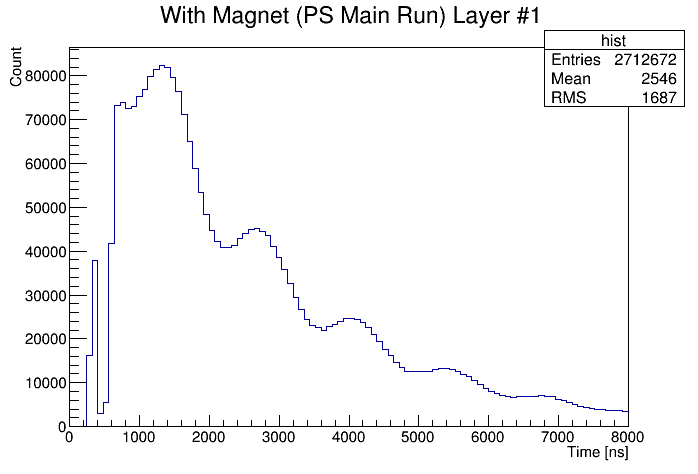
\includegraphics[width = 0.45\textwidth]{figure/odagawa/PSgFactorDist_Layer0.eps}\\
	\begin{minipage}{0.45\textwidth}
	\centering
	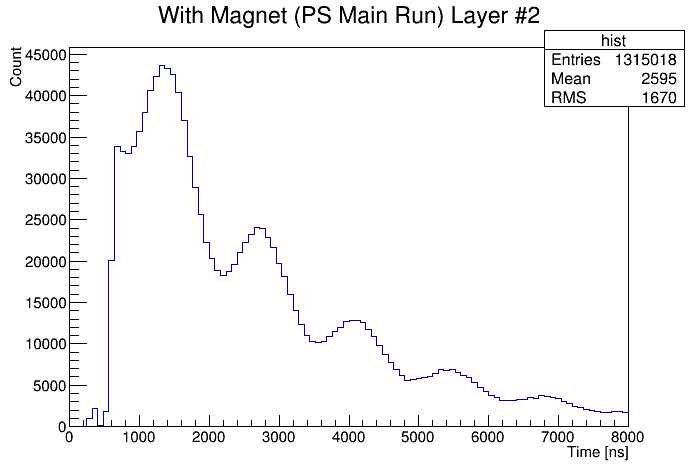
\includegraphics[width = \textwidth]{figure/odagawa/PSgFactorDist_Layer1.eps}
	\end{minipage}
	\begin{minipage}{0.45\textwidth}
	\centering
	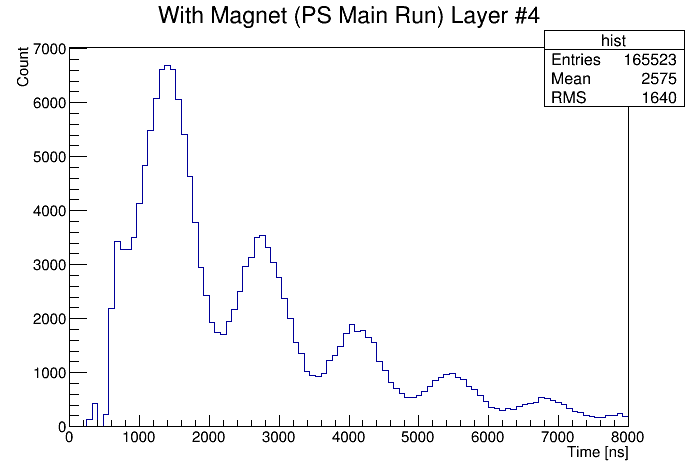
\includegraphics[width = \textwidth]{figure/odagawa/PSgFactorDist_Layer3.eps}
	\end{minipage}
	\caption{磁場があるときの時刻分布ヒストグラム.それぞれ (上) 1 層目,(左下) 2 層目コインシデンスあり,(右下) 4 層目コインシデンスありのものである.指数関数減衰にミューオンの歳差運動由来と思われる振動が重なっている.}
	\label{fig:PSgFactorDist}
\end{figure}%

図~\ref{fig:PSgFactorDist} のヒストグラムに%式\eqref{eq:PSgFactorFitFunc}
\begin{equation}
g(t) = A \exp(-t / \tau) [1 + B \cos(\delta + \omega t)] + \mathrm{const.}
\label{eq:PSgFactorFitFunc}
\end{equation}
で表される関数$g(t)$ を用いてフィッティングを行った.
ここで\ref{subsubsec:PSLife} のときと同様に定数項を加え,フィッティング範囲を振動がきちんと見えている1000~ns から8000~ns までとした.
フィッティング結果を図~\ref{fig:PSgFactorFit},および表\ref{tab:PSgFactor} に示す.
ただし表~\ref{tab:PSgFactor} において$g$ 因子の計算には各点の磁場をビームプロファイルのガウシアンで加重平均した値,$B = 53.97~\mathrm{G}$ という値を用いた.
また,誤差としては\ref{subsubsec:PSLife} と同様にフィッティングの統計によるものを載せており,磁場の影響を含めたものについては後述する.
\begin{figure}[h]
	\centering
	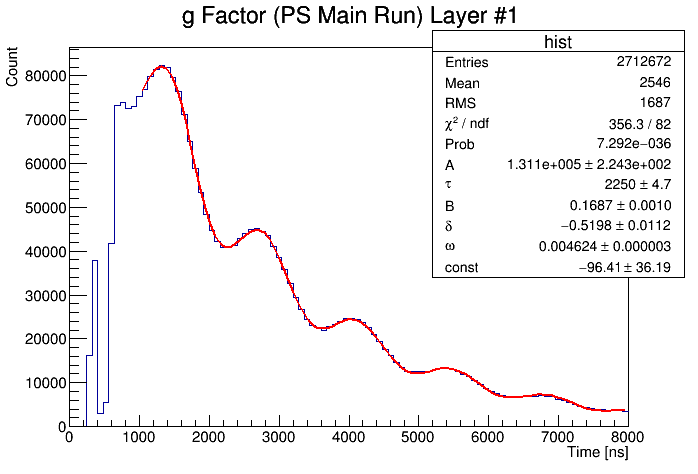
\includegraphics[width = 0.45\textwidth]{figure/odagawa/PSgFactorFit_Layer0.eps}\\
	\begin{minipage}{0.45\textwidth}
	\centering
	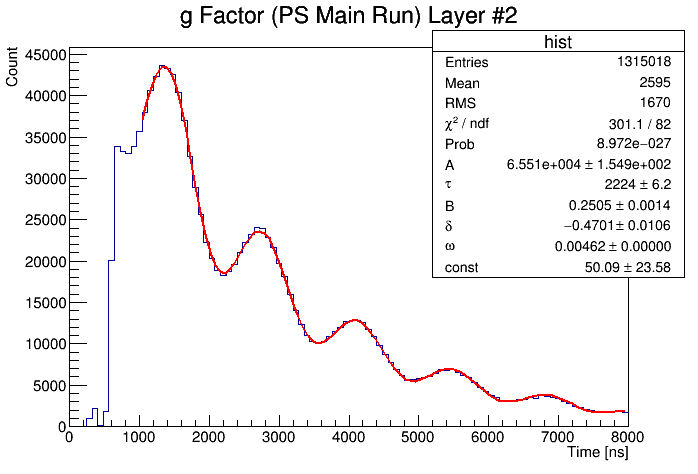
\includegraphics[width = \textwidth]{figure/odagawa/PSgFactorFit_Layer1.eps}
	\end{minipage}
	\begin{minipage}{0.45\textwidth}
	\centering
	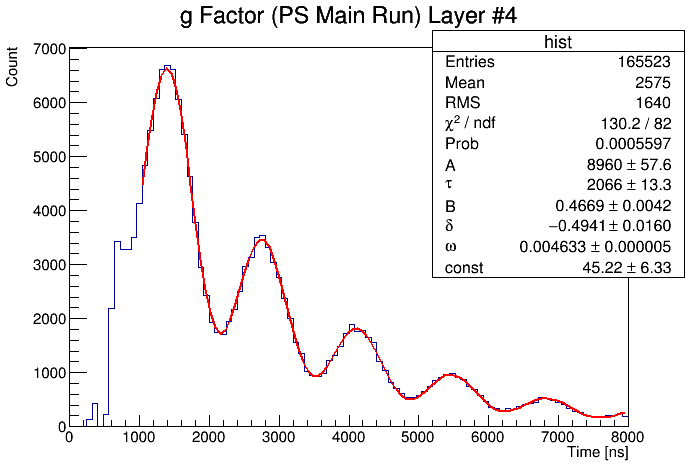
\includegraphics[width = \textwidth]{figure/odagawa/PSgFactorFit_Layer3.eps}
	\end{minipage}
	\caption{図~\ref{fig:PSgFactorDist} のヒストグラムに$g(t)$ でフィッティングを行った結果.それぞれ (上) 1 層目,(左下) 2 層目コインシデンスあり,(右下) 4 層目コインシデンスありのものである}
	\label{fig:PSgFactorFit}
\end{figure}%
\begin{table}[h]
	\centering
	\caption{$g$ 因子フィッティング結果}
	\begin{tabular}{cccc} \toprule
	層番号 & $\tau~[\mathrm{ns}]$ & $\omega~[/ \mu\mathrm{s}]$ & $g$ \\ \midrule
	1 & $2249 \pm \phantom{0}4$ & $4.624 \pm 0.004$ & $2.013 \pm 0.0015$ \\  
	2 & $2224 \pm \phantom{0}6$ & $4.620 \pm 0.003$ & $2.012 \pm 0.0015$ \\  
	4 & $2066 \pm 13$ & $4.633 \pm 0.005$ & $2.017 \pm 0.0023$ \\  \bottomrule
	\end{tabular}\label{tab:PSgFactor}
\end{table}%

さらに磁場測定機器の測定誤差を含んだ$g$ 因子の統計誤差については,誤差伝播の式,式\eqref{eq:PSgosa} を用いて計算した.
\begin{equation}
\delta g = \sqrt{\left(\delta\omega\right)^{2}\left(\frac{\partial g}{\partial\omega}\right)^{2} + \left(\delta B\right)^{2}\left(\frac{\partial g}{\partial B}\right)^{2}}
\label{eq:PSgosa}
\end{equation}%
$\delta B = 2.36~\mathrm{G}$となったので,$\delta g$ は表~\ref{tab:PSgStatErr} のようになった.
\begin{table}
	\centering
	\caption{磁場測定機器の測定誤差を含んだ$g$ 因子の統計誤差}
	\begin{tabular}{cc}\toprule
	層番号 & $g$ 因子の統計誤差\\ \midrule
	1 & 0.008 \\ 
	2 & 0.008 \\
	4 & 0.009 \\ \bottomrule
	\end{tabular}\label{tab:PSgStatErr}
\end{table}%

\subsubsection{磁場の系統誤差について}
\label{subsubsec:MagSysErr}

\ref{subsubsec:PSgFactor} において$g$ 因子解析に用いた磁場の値$B = 53.97~\mathrm{G}$ は事前にMLF の三宅さんから頂いたビームプロファイルをもとに加重平均をとった値であるが,このビームプロファイルの不定性により加重平均の値は変化する.
今回はビームの広がりはガウシアンにしたがって分布すると仮定したうえでガウシアンの広がりを変化させ,それによる磁場への影響をみた.

ガウシアンの$x$ 方向の広がりを$\sigma_{x}$,$y$ 方向の広がりを$\sigma_{y}$ とし,$\sigma_{x}$ を2.0~cm から3.9 ~cm まで,$\sigma_{y}$ を1.0~cm から2.9~cm まで0.1~cm 刻みで変化させて加重平均磁場の値を求めた.得られた2 次元分布を図~\ref{fig:PSMagMinMax} に,その最大値・最小値を表~\ref{tab:MagSysErr} に示す.ここで用いた磁場の値はすべて表~10のものである.
$\sigma_{x}, \sigma_{y}$ を動かす範囲は磁場標的の大きさが事前にいただいたビームプロファイルのガウシアンの標準偏差$1\sigma$ に入る点を上限として十分な広さをとった.
\begin{figure}[h]
	\centering
	\includegraphics[width = 0.9\textwidth]{figure/odagawa/magminmax.eps}
	\caption{$\sigma_{x}, \;\sigma_{y}$ を0.1~cm 刻みで動かしたときの磁場の加重平均の値.中心付近の点はいただいていたビームプロファイルでの値を示している.最大値をとったのは$\sigma_{x} = 3.9, \;\sigma_{y} = 1.0$ のとき,最小値をとったのは$\sigma_{x} = 3.9, \;\sigma_{y} = 2.9$ のときであった.}
	\label{fig:PSMagMinMax}
\end{figure}
\begin{table}[h]
	\centering
	\caption{$\sigma_{x}$,$\sigma_{y}$を動かしたときの磁場$B$ の最大値と最小値~[G]}
	\begin{tabular}{cc}\toprule
	$B_{\mathrm{max}}$ & $B_{\mathrm{min}}$ \\ \midrule
	$54.44 (\sigma_{x} = 3.9, \;\sigma_{y} = 1.0)$ & $53.76 (\sigma_{x} = 3.9, \;\sigma_{y} = 2.9)$ \\ \bottomrule 	
	\end{tabular}\label{tab:MagSysErr}
\end{table}%

得られた磁場の最大値,および最小値を用いて計算した$g$ 因子の値を表~\ref{tab:PSgSysErr} に示す.
\begin{table}[h]
	\centering
	\caption{磁場$B$ の値とそれらに対応する$g$ 因子の値}
	\begin{tabular}{cccc}\toprule
	層番号 & $B_{\mathrm{max}} = 54.44~\mathrm{G}$ & $B_{0} = 53.97~\mathrm{G}$ & $B_{\mathrm{min}} = 53.76~\mathrm{G}$ \\ \midrule
	1 & 2.000 & 2.013 & 2.021 \\
	2 & 1.995 & 2.012 & 2.020 \\
	4 & 2.000 & 2.017 & 2.025 \\ \bottomrule 
	\end{tabular}\label{tab:PSgSysErr}
\end{table}%

実際,$g$ 因子の値を考えるときは1 層目と4 層目とのコインシデンスをとったものが銅板にミューオンがあたった上で検出器に飛来したような貫通イベントをとれている可能性が高く磁場の影響を受けた$e^{+}$ が多いと考えられることからも妥当であると考えると,得られた$g$ 因子の値は
\[g = 2.017 \pm 0.009 ^{+0.008}_{-0.017}\]
となった.
ここで誤差の第一項は統計誤差であり,第二項はビームプロフィルの不定性による系統誤差である.

%以下二つはAppendix にまわす?
%%%%%%%%%%%%%%%
\subsubsection{磁場の変化の確認}
\label{subsubsec:PSMagChangeCheck}

$g$ 因子測定のための磁場標的を置いたランの途中で磁石配置が崩れ,磁場の値が変わっていたことは本文中でも述べたが,解析においてそのことを確認した.

\ref{subsubsec:PSgFactor} のようなフィッティングをする際に,用いるイベントを9000~events (6~min) ごとに区切ってフィッティングを行った,それぞれ得られた$\omega$ をの値を図~\ref{fig:PSOmegaCheck} に示す.
赤線は最初の8~分間のデータから得られた値を表しており,また青線は磁場変化発覚後に改めて確認用にとったランから得られた値を表している.
ここで磁場変化発覚後のランはおよそ30~分間である.図~\ref{fig:PSOmegaCheck} を見ると分かるように,ランの最初の20~分程度で磁場の値が変化している.
よって今回の解析には同じ値の磁場とみなせるという条件の下で,より統計量の多いランの20~分以降のデータを用いることにした.
なお,変化前後の加重平均をとった磁場の値はそれぞれ56.06~G と53.97~G であった.
\begin{figure}[h]
	\centering
	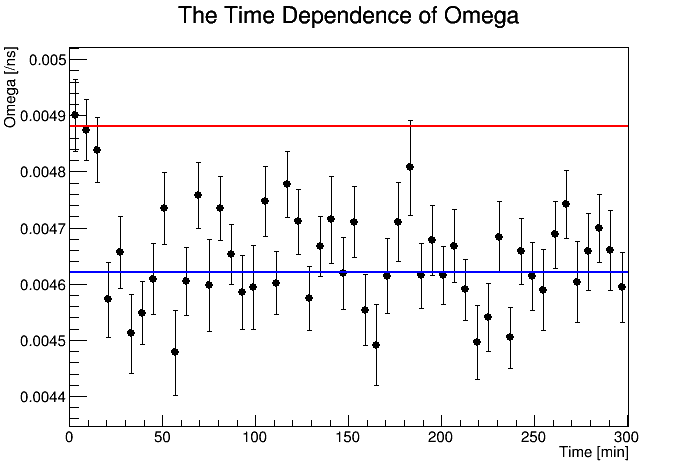
\includegraphics[width = 0.9\textwidth]{figure/odagawa/PSOmegaCheck.eps}
	\caption{ラン中における$\omega$ の時間変化.最初の20~分間を過ぎたあたりから$\omega$ の値が変化している様子が見られる.}
	\label{fig:PSOmegaCheck}
\end{figure}

\subsection{PS の解析まとめ}
\label{subsec:PSmatome}

二つの解析手法を用いてミューオンの寿命,および$g$ 因子を求めた.これらの結果を表~\ref{tab:matome_PS} にまとめた.
\begin{table}[h]
	\centering
	\caption{二つの手法によるプラスチックシンチレータでの解析結果}
	\begin{tabular}{ccc}\toprule
	{} & 解析手法A & 解析手法B \\ \midrule
	$\tau$~[ns]& $2227 \pm 5_{- 53}$ & 2220 $\pm$ 18\\
	$g$ & $2.005 \pm 0.003^{+0.018}$  & $2.017 \pm 0.009 ^{+0.008}_{-0.017}$\\ \bottomrule
	\end{tabular}\label{tab:matome_PS}
\end{table}%

%二つの解析結果をまとめると,表~\ref{tab:matome_PS2} のようになった.ここでそれぞれの系統誤差はそのまま含めた.

%\begin{table}[H]
%	\centering
%	\caption{二つの解析結果をまとめた値}
%	\begin{tabular}{cc}\toprule
%	$\tau$~[ns]& $2222 \pm 9_{-75}$\\
%	$g$ & $2.010 \pm 0.005 \pm 0.017$\\ \bottomrule
%	\end{tabular}\label{tab:matome_PS2}
%\end{table}%

%\end{document}
